\documentclass[a4paper]{article}

%--------------------------------------------------------------------------
\usepackage[a4paper, total={6in, 8in}]{geometry}
\usepackage{booktabs}
\usepackage{graphicx}
\usepackage{listings}
\usepackage{siunitx}

%--------------------------------------------------------------------------
\graphicspath{{./fig}}

%--------------------------------------------------------------------------
\begin{document}
\title{Udacity: Search and Sample Return Report}
\author{Shane Reynolds}
\maketitle
%--------------------------------------------------------------------------
\section{Introduction \& Background}
A simplistic and wide reaching definition of a robot is a machine which performs a task with some level of autonomy. In this context, robotic systems are appealing as they allow humans to avoid work that is considered dull, dirty and dangerous. This broad definition somewhat obfuscates the elements that make robotics work. Indeed, there is no clear consensus as to the mandatory sub-systems which comprise a robotic system, however, there are some common features which can be observed across many existing robotics platforms, these include:
\begin{itemize}
\item \textbf{Perception systems}: systems which allow the robot to perceive the world around it
\item \textbf{Decision making systems}: systems which allow the robot to decide a course of action given some information set
\item \textbf{Actuation systems}: systems which allow the robot to physically interact with the world
\end{itemize}

This project serves as a short introduction to these three systems. Principally, it touches on elementary image processing concepts, and very briefly explores some basic decision making. The project is based on a simulated mobile robot operating in a simple terrain environment. The simulation is built in Unity and main python script which gives the robot perception and decision making capabilities is called XXXX. Finally, the interface between image processing, decision making algorithms, and the simulation is driven by SocketIO. A screen shot of the simulation can be seen in Figure 1 below.

\begin{figure}
\centering
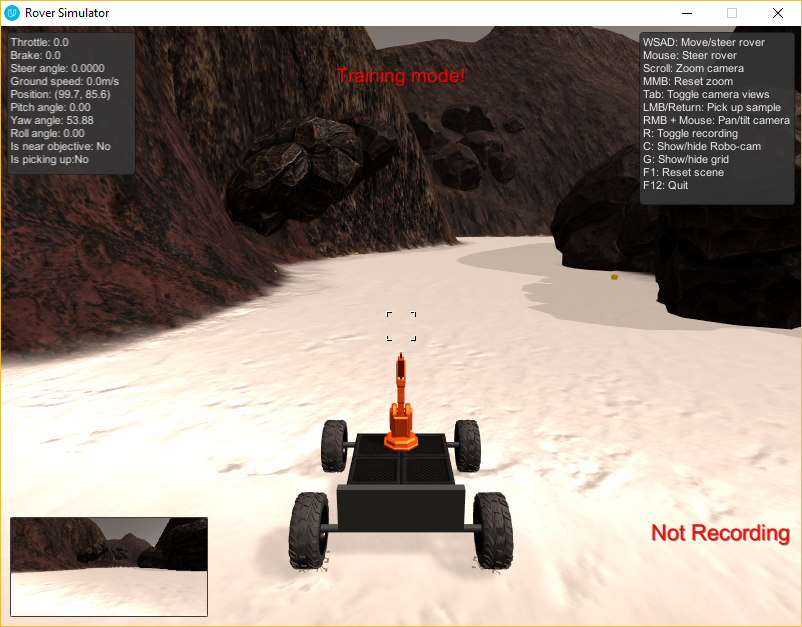
\includegraphics{image1}
\caption{A screenshot of the mobile robotic rover at a standstill in the simulated environment.}
\end{figure}

%--------------------------------------------------------------------------
\section{Methods and Implementation}
\subsection{Sensor Data}
The robot perceives its world via sensors. The main sensor used in this project is the camera mounted to the front of the robot. Figure 2 shows an example of a single image captured from the rover's camera. The camera images are received approximately once every 27$\si{\milli\second}$, or 36$\si{\hertz}$.

\begin{figure}
\centering
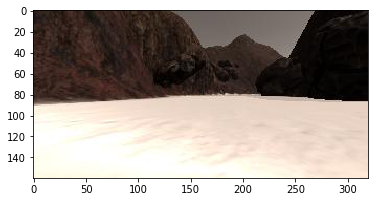
\includegraphics{image2}
\caption{A single image of the simulated environment as shown from the robot's front mounted camera.}
\end{figure}

In addition to the camera data, the there are sensors which measure the rover's position and orientation in space. Position is given by simple Cartesian coordinates, $(x, y)$, with reference to a fixed world frame. Orientation is given by roll, pitch, and yaw which are also with reference to the fixed world frame. Finally, throttle, brake, and steering angle of the rover are also provided. These values values are received at the same frequency as the images. The sensor data is used to help determine a course of action for the robot. This is achieved with two principal functions: \verb|perception_step| and \verb|decision_step|. Table 1 shows the different sensors data types, and a basic description of use of the captured data. 

\begin{table}
\caption{A table which shows the different sensor data types, and their python format.}
\begin{tabular}{lll}
\toprule
\textbf{Sensor Data Type} & \textbf{Python Variable} & \textbf{Description}\\
\midrule
Image & \verb|img| & This is the \\
Position & \verb|pos| & value\\
Yaw & \verb|yaw| & \\
Pitch & \verb|pitch| & \\
Roll & \verb|roll| & \\
Current Velocity & \verb|velocity| & \\
Steering Angle & \verb|steer| & \\
Throttle Value & \verb|throttle| & \\
Brake Value & \verb|brake| & 
\bottomrule
\end{tabular}
\end{table}

%--------------------------------------------------------------------------
\subsection{Image Processing}
The image processing was a large component of the project, and consisted of multiple stages. Image processing is applied by the \verb|perception_step| function, and is applied to each image captured by the rover's front mounted camera. The processing consists of three principal components: perspective transformation, segmentation, and translating the image to obtain a rover centric coordinate system. There is no fixed order in which the perspective transformation and segmentation steps need to occur, however, the transformation to a rover centric coordinate system can only be performed once the image has undergone a perspective transformation.


%--------------------------------------------------------------------------
\subsubsection{Perspective Transformation}
Describe the implementation of how the image transformation was made. Basically, we obtained 4 points on the received image, and 4 points on the overhead image. We map the points from the front facing camera image to the overhead image for the rover in a given position. This mapping is done manually using image viewer

\begin{lstlisting}[language=]

\end{lstlisting}

\begin{table}
\caption{include a table which has the points that we need to map to the other points}
\begin{tabular}{content...}
content...
\end{tabular}
\end{table}

\begin{figure}
\begin{minipage}{0.45\linewidth}
\centering
\caption{include an image from the front facing camera}
\end{minipage}
\begin{minipage}{0.45\linewidth}
\centering
\caption{include an image from the overhead camera}
\end{minipage}
\end{figure}

\begin{figure}
\begin{minipage}{0.45\linewidth}
\centering
\caption{include a graphic of the transformation being applied - original image}
\end{minipage}
\begin{minipage}{0.45\linewidth}
\centering
\caption{include a grapic of the transformation being applied - transformed image}
\end{minipage}
\end{figure}

\subsubsection{Segmentation: Navigable Terrain \& Obstacles}
There are 3 different types of object that are of interest to the robot: navigable terrain, obstacles, rock samples. A simple way to obtain the navigable terrain is to create a basic RGB filter. This works because it exploits the stark contrast between obstacles (which are dark), and navigable terrain (which is light). We get two for one with this type of filtering if we can filter the navigable terrain, then we have the obstacles by default - that is the two types of terrain are mutually exclusive.

CODE SNIPPET

\begin{figure}
\begin{minipage}{0.45\linewidth}
\centering
\caption{Include a grpahic of the original image}
\end{minipage}
\begin{minipage}{0.45\linewidth}
\centering
\caption{Include a graphic of the terrain being filtered - gray scale}
\end{minipage}
\end{figure}

This section is more curious that that. If we filter prior to transforming, then there is some distortion to the filtered image. Basically determined what the cone is and subtracted this from the transformation to ge the final image. Further, some spacing has been left in between the navigable terrain and the obstacles to provide for a margin of error.

\begin{figure}
\centering
\caption{include a graphic of the final terrain being filtered for obstacles and }
\end{figure}

PERHAPS TEST: see what happens if the segmentation is made first and then the transformation is made leaving an image gap - if there is no distortion then this may be the better solution.

\subsubsection{Segmentaiton: Rock Samples}
To get the rock samples it was a little harder - the RBG did not work that well and instead HSV was used. Talk some about the RGB background and then talk some about the HSV background. Once the rocks have been determined they are added to the image

CODE SNIPPET

\begin{figure}
\begin{minipage}{0.45\linewidth}
\centering
\caption{include a graphic of the original rock image}
\end{minipage}
\begin{minipage}{0.45\linewidth}
\centering
\caption{include a graphic of the filtered image - gray scale}
\end{minipage}
\end{figure}

\begin{figure}
\centering
\caption{Include an image of the full image transformation with the rock and the blue and green}
\end{figure}

\subsubsection{Rover Centric Coordinates}
Transformation of the image into a rover centric coordinate frame. The transformed image needs to be attached to the rover centric coordinate frame - this needs more explaining exactly what is happening here with the transformed image. What is it doing and why do we do it?

CODE SNIPPET

\begin{figure}
\begin{minipage}{0.45\linewidth}
\centering
\caption{include a non-transformed image}
\end{minipage}
\begin{minipage}{0.45\linewidth}
\centering
\caption{include an image of the transformed rover centric coord system}
\end{minipage}
\end{figure}

\subsubsection{Writing Colour Map to the World Map}

Updates the map. Describe what is actually happening here? This has not yet been described - essentially what we have is an image and we want to update the ground truth of the world map as the rover explores autonomously.

CODE SNIPPET

\begin{figure}
\centering
\caption{Show a picture of the mapped terrain, if possible}
\end{figure}

%--------------------------------------------------------------------------
\subsection{Autonomous Navigation}
\subsubsection{Perception Step}
Need to talk about the implementation of these sections of the code

\subsubsection{Decision Step}
Need to talk about the implementation of these sections of the code

%--------------------------------------------------------------------------
\section{Results \& Conclusion}

%--------------------------------------------------------------------------
\section{Further Enhancements}

\end{document}